
% ??ds make sure TR and BDF2 are mentioned before this chapter or add refs here!
% ??ds similarly for "semi-discretised"
% " for order of a time integrator

% In the plots:
% add points

\chapter{An adaptive implicit midpoint rule time integrator}
\label{sec:adaptive-imr}


The implicit midpoint rule (IMR) is a well known time integration method with a number of favourable properties when applied to standard ordinary differential equations\cite[204]{HairerNorsettWanner}.
It also has beneficial ``geometric integration'' properties when applied the Landau-Lifshitz-Gilbert equation (discussed in \autoref{sec:aimr-llg}) and energy conservation properties when applied to the semi-discretised Navier-Stokes equations \cite{Sanderse2013}.
However IMR belongs to the implicit Runge-Kutta family of methods, and as such it is a non-trivial task to create an efficient adaptive time step selection algorithm.
In this \secpaper{} we describe a novel adaptive IMR algorithm based on estimates of the local truncation error by a predictor step.


\section{Implicit midpoint rule with fixed step size}
\label{sec:fixed-step-implicit}

Let $\yv(t)$ be a vector function and denote an approxmimation to $\yv(t)$ at $t = t_n$ by $y_n$.
Let $\dtn = t_{n+1} - t_n$ be the $n$th time step (or just ``step'').
Then given a system of ordinary differential equations (ODEs) of the form
\begin{equation}
  \yv'(t) = \ffv{t, \yv(t)},
  \label{eq:43}
\end{equation}
the implicit midpoint rule (IMR) is
\begin{equation}
    \yv_{n+1} = \yv_n + \dtn \ffv{\frac{t_{n+1} + t_n}{2}, \frac{\yv_n + \yv_{n+1}}{2}}.
\end{equation}

We introduce some notation for the midpoint values of $t$ and $\yv$:
\begin{equation}
  \begin{aligned}
    \thf & = \frac{t_{n+1} + t_n}{2} \quad \bigb{= t_n + \frac{\dtn}{2}}, \\
    \yvm &= \frac{\yv_{n+1} + \yv_n}{2}.
  \end{aligned}
\end{equation}
In this notation the IMR is
\begin{equation}
  \yv_{n+1} = \yv_n + \dtn \ffv{\thf, \yvm}.
  \label{eq:basic-midpoint}
\end{equation}

The IMR can also be written in the standard form for Runge-Kutta methods as
\begin{equation}
  \begin{aligned}
    k_1 &= \ffv{t_n + \frac{1}{2} \dtn, \yv_n + \frac{1}{2} k_1}, \\
    \yv_{n+1} &= \yv_n + 1 \cdot \dtn k_1,
  \end{aligned}
\end{equation}
or using a Butcher tableu \cite[135]{HairerNorsettWanner} as shown in \autoref{tab:butcher-imr}.

\begin{table}
  \begin{equation*}
    \begin{array}{c|c}
      \frac{1}{2}  &     \frac{1}{2}  \\
      \hline
                   & 1 \\
    \end{array}
  \end{equation*}
  \caption{The Butcher tableu for the implicit midpoint rule.}
  \label{tab:butcher-imr}
\end{table}

Note that unlike multistep methods, such as the second order backwards difference (BDF2), \eqref{eq:basic-midpoint} is valid for both constant and variable step sizes because there is no dependence on previous steps.

Next we discuss some properties of IMR applied to ODEs and compare them to some other widely used time integration methods.
We compare with BDF2 and the trapezoid rule (TR), because they have very similar stability, accuracy and computational cost to IMR.


\subsection{Local truncation error and order}
\label{sec:deriv-local-trunc}

The local truncation error (LTE) of a time integration scheme is the error due to a single integration step.
It can be calculated by substituting $\yv_n = \yv(t_n)$ into the approximation for the next time-step then subtracting the result from the exact solution at the next time-step, $\yv(t_{n+1})$. 
\ie
\begin{equation}
  \lte = \yv(t_{n+1}) - \hat{\yv}_n,
\end{equation}
where the history values ($\yv_{n-1}, \yv_{n-2}, \ldots$) used to calculate $\hat{\yv}_n$ are exact.
??ds can we write this more rigorously? Write $y_n$ as a function of history values?

Using this definition the local truncation error of IMR is
\begin{equation}
  \lte^\imr =  \yv(t_{n+1}) - \yv(t_n) - \dtn \ffv{\thf, \frac{\yv(t_n) + \yv_{n+1}^\imr}{2}}.
  \label{eq:trunc-start}
\end{equation}

It is important to distinguish the local truncation error from the global (temporal) error
\begin{equation}
  \label{eq:global-temporal-error}
  \begin{aligned}
    E_n^\imr &= \yv(t_{n+1}) - \yv_{n+1}^\imr, \\
    &=  \yv(t_{n+1}) - \yv_n^\imr - \dtn \ffv{ \thf, \frac{\yv_n^\imr + \yv_{n+1}^\imr}{2} }.
  \end{aligned}
\end{equation}
The difference is that the global error includes any error accumulated over previous time steps (the exact values $\yv(t_n)$ in \eqref{eq:trunc-start} are replaced by their approximations).

We now expand the IMR local truncation error into a more useful form.
We first Taylor expand $\yv(t_{n+1})$ and $\yv(t_{n})$ about $\thf$.
We use the midpoint rather than one of the end points (as typically used in these calculations) because it results in simpler calculations.
Assuming that $\yv(t)$ is ``sufficiently smooth'' for the required derivatives to exist its Taylor series expansion at $t_{n+1}$ about $\thf$ is given by
\begin{equation}
  \yv(t_{n+1}) = \yv(\thf + \frac{\dtn}{2}) = \yvhf + \frac{\dtn}{2} \yvhf['] 
  + \frac{\dtn^2}{8} \yvhf['']
  + \frac{\dtn^3}{48} \yvhf[''']
  \porder{\dtn^4}.
  \label{eq:taylornp1}
\end{equation}
Similarly the expansion at $t_n$ about $\thf$ is
\begin{equation}
  \yv(t_n) = \yv(\thf - \frac{\dtn}{2}) = \yvhf - \frac{\dtn}{2} \yvhf['] 
  + \frac{\dtn^2}{8} \yvhf[''] 
  - \frac{\dtn^3}{48} \yvhf['''] 
  \porder{\dtn^4}.
  \label{eq:taylorn}
\end{equation}

Substituting equations~\eqref{eq:taylornp1} and \eqref{eq:taylorn} into equation~\eqref{eq:trunc-start} gives\footnote{If we had chosen to Taylor expand about $t_n$ there would be an additional term in $\yv_n''$ here.}
\begin{equation}
  \lte^\imr = \underbrace{\frac{\dtn^3}{24} \yvhf[''']}_{\text{I}}
  + \underbrace{\dtn\bigs{ \yvhf['] - \ffv{\thf, \frac{\yv(t_n) + \yv_{n+1}}{2}} }}_{\text{II}}
  \porder{\dtn^4}.
  \label{eq:trunc-mid}
\end{equation}

There are two parts to this error: the first term (I) is fairly standard in second order time integrators.
The second term (II) originates from the use of an approximation to $\yv(\thf)$ in the evaluation of $\fv$ (\ie the Runge-Kutta nature of IMR).
The rest of the derivation requires applying Taylor expansions to II and is carried out in \autoref{sec:full-imr-lte-calculation}.
The final result shows that IMR is second order:
\begin{equation}
  \lte^\imr = \frac{\dtn^3}{24} \left[\yvhf['''] - 3 \dfdyhf \cdot \yvhf[''] \right]
  \porder{\dtn^4},
  \label{eq:trunc-final}
\end{equation}
where $\dfdyhf = \pd{\fv}{\yv}\evalat{t=\thf}$ is the Jacobian of $\fv$ with respect to $\yv$ evaluated at $t=\thf$.
An additional condition required in the derivation is that ??ds the eigenvalues of $\dtn\dfdyhf$ are less than one, the implications of this are discussed in \autoref{sec:order-reduction}.

The TR\cite[261]{GreshoSani} and BDF2\cite[715]{GreshoSani} methods are also second order.
Their local truncation errors are similar to I:
\begin{equation}
  \label{eq:tr-lte}
  \lte^\tr = \yv_{n+1} - \yv(t_{n+1}) = -\frac{\dtn^3 \yv_n'''}{12}
  + \order{\dtn^4},
\end{equation}

\begin{equation}
  \label{eq:bdf2-lte}
  \lte^\bdf = \yv_{n+1} - \yv(t_{n+1}) = \frac{(\dtn + \dtx{n-1})^2}{\dtn(2\dtn + \dtx{n-1})}
  \frac{\dtn^3 \yv_n'''}{6}
  + \order{\dtn^4}.
\end{equation}


\subsection{A-stability}

To discuss the stability of time integrators for stiff problems the following test equation is widely used
\begin{equation}
  \ffv{\yv} = \lambda \yv,
  \label{eq:ode-test-f}
\end{equation}
\ie
\begin{equation}
  \yv(t) = \exp(\lambda t).
\end{equation}

A-stablility\footnote{The A does not stand for anything, it is just ``A''\cite[40]{HairerWanner}, in particular it does \emph{not} mean ``absolute stabilily''.} is the property that a method is has no stability restrictions on the time step size when used to integrate \eqref{eq:ode-test-f} for all $\lambda$ with $\realp(\lambda) \leq 0$.
When $\realp(\lambda) > 0$ the ODE itself is unstable and so stability is not expected in general.
A-stability is a good way to classify the suitability of a time integrator for solving stiff ODEs (such as those that often emerge from a semi-discretisation of a PDE).

The IMR, TR, BDF1 and BDF2 methods are all A-stable \cite[pgs. 43, 251]{HairerWanner}.
Linear explicit methods are never A-stable \cite{Nevanlinna1974} (``linear'' methods include all common time integration methods: Runge-Kutta, linear multistep, predictor-corrector...)\footnote{These limitations could potentially be circumvented by using non-linear methods, such methods are beyond the scope of this thesis.}, which is the main reason for our focus on implicit methods.


\subsection{L-stability and numerical damping}
\label{sec:imr-l-stability}

L-stability is another stability property beyond A-stability.


\begin{equation}
  \lim_{z=h\lambda \goesto \infty} y_1/y_0 = 0,
\end{equation}
??ds fill this in

Property that method damps oscillations a bit.

IMR and TR are not L-stable, BDF1 is \cite[45]{HairerWanner}. BDF2 probably is citation elsewhere?

L-stability is both a positive and negative property: if the oscillations being damped are spurious then L-stability can increase accuracy of the solution \cite[45]{HairerWanner}.
However the same property results in the damping of non-spurious oscillations, this can cause problems (see e.g. \autoref{fig:bdf2-failing on switching nanoparticle}, \cite[242]{GreshoSani}, \cite{Elman2011}.


\subsection{B-convergence and order reduction}
\label{sec:order-reduction}

It is known that certain implicit Runge-Kutta methods are susceptible to reduced accuracy when used to solve certain extremely stiff problems \cite[156]{Atkinson1994}\cite[225]{HairerWanner}.
In the case of the implicit midpoint rule this corresponds to the case when the error due to term II of \eqref{eq:trunc-mid} is large. This occurs when $\pd{\fv}{\yv}\evalat{\thf{}}$ is large, \ie when the change in $\ffv{t, \yv}$ due to a small error in $\yv$ is large.

The concept of ``B-convergence'' is used to analyse this effect.
Roughly speaking a Runge-Kutta method is B-convergent of order $r$ if the global error is  $\order{\dtx{\text{max}}^r}$ for all sufficiently smooth ODEs without any assumption about the size of $\pd{\fv}{\yv}$.
The implicit midpoint rule is B-convergent of order 1 \cite[231]{HairerWanner}, one order less than for typical ODEs.
In contrast, the TR and BDF methods do not suffer from order reduction \cite[159]{Atkinson1994}\footnote{In this book IMR is refered to as the second order Gauss method, BDF1 is Radau IIA, TR is Lobatto IIIA \cite[72-76]{HairerWanner}.}.
This is because all evaluations of $\fv$ are at integer time points (\ie $t_{n+1}, t_{n}, t_{n-1}, \ldots$ rather than $\thf$).

A simple test ODE gives a useful example of this phenomenon \cite[157]{Atkinson2009}
\begin{equation}
  \label{eqn:imr-test-order-reduction}
  \begin{aligned}
    f(t, y) &= -\lambda (y - g(t)) + g'(t), \\
    y(t) &= g(t), \\
  \end{aligned}
\end{equation}
for some function $g(t)$ and parameter $\lambda \geq 0$.
Note that $\pd{f}{y} = \lambda$, so we can directly control the second term of the IMR truncation error.

We now derive the LTE for IMR in this example when $\abs{\lambda\dtn} >> 1$.
From \autoref{sec:full-imr-lte-calculation}, \eqref{eq:trunc-implicit-form} we have that
\begin{equation}
  \begin{aligned}
    (1 + \frac{\dtn \lambda}{2})\lte^\imr &= \frac{\dtn^3}{24}
    \bigs{g'''(\thf) - 3 \lambda g''(\thf)} \porder{\dtn^4}, \\ 
  \end{aligned}
\end{equation}
Then using $\abs{\lambda\dtn} >> 1$:
\begin{equation}
  \begin{aligned}
    \frac{\dtn \lambda}{2} \lte^\imr &= \frac{\dtn^3}{24}
    \bigs{g'''(\thf) - 3 \lambda g''(\thf)} \porder{\dtn^4}, \\ 
    \lte^\imr &= \frac{\dtn^2}{12\lambda} \left[g'''(\thf) - 3 \lambda g''(\thf) \right] \porder{\dtn^4}.
  \end{aligned}
\end{equation}
So we can see that the order has been reduced by a factor of $1/\dtn$.
If addtionally $\abs{\lambda\dtn} >> \abs{g'''(t)}$, which will typically be true for very large $\lambda$ and $g \neq g(\lambda)$:
\begin{equation}
  \lte^\imr = \frac{-\dtn^2}{4} g''(\thf).
  \label{eq:reduced-order-imr-truncation-error}
\end{equation}

This order reduction effect should be automatically detected and adjusted for by a good adaptive time step selection algorithm.


% The IMR and the BDF1 methods are B-convergent, TR is not B-convergent, the BDF2 method does not fit into the framework used to analyse such methods\cite[231]{HairerWanner}.



\section{Construction of an LTE estimate}

Most local truncation error estimators for implicit integrators (e.g. trapezoid rule, BDF2) use a Milne-device based method \cite[707-716]{GreshoSani}.
This means that they compute an explicit estimate $\yv^E_{n+1} \sim \yv(t_{n+1})$  (sometimes known as a predictor step) to the same order of accuracy as the implicit method and using the same input values and derivatives.
They then use algebraic rearrangements of the LTE expressions of the predictor step and the real step to give approximation of the LTE.

However due to the complexity of the local truncation error of the implicit midpoint rule there are difficulties with this approach.
In particular, the LTE of IMR has a term involving the error due to the approximation $\yv(\thf) \sim \yvm$.
In order to perform the algebraic rearrangements to obtain the LTE we need the this term to appear in the LTE of the predictor.
However it can only appear in the LTE expression for a time integrator using midpoint approximation, and the only such second order time integrator is IMR itself.
So this term of the error cannot be easily approximated using a Milne-device-like method.

An alternative approach, commonly used in Runge-Kutta time integrators, is to repeat the calculation using a higher order method and compare the two answers to directly obtain an LTE estimate \cite[165]{HairerWanner}.
However evaluations of the derivative function ($\fv$ in equation~\eqref{eq:43}) are expensive, and the calculation of a step of a high order Runge-Kutta method requires a number of function evaluations.
Hence such approaches usually rely on pairs of Runge-Kutta methods which share most of their derivative evaluation points but have different orders of accuracy.
These are known as embedded Runge-Kutta methods, a widely used example is the Dormand–Prince pair (order 4/5) used in MATLAB's \texttt{ode45} function \cite{matlab-ode45}.

Unfortunately there is no third order method which uses $\ffv{\thf, \yvm}$ and one other function evaluation.\footnote{IMR's single function evaluation is positioned such that the second order error terms cancel. Adding one additional evaluation cannot retain the symmetry causing this cancellation and so does not increase the order.}
To get around this problem we instead use a little known explicit version of the third order backwards difference method (eBDF3) instead of using a higher order Runge-Kutta method.
This requires only 3 history values and a single explicit function evaluation in order to compute a 3rd order accurate approximation to $\yv(t_{n+1})$.
Since only one function evaluation is required this is roughly as efficient as an embedded Runge-Kutta method without the requirement to reuse the existing function evaluations.
With this approach our estimate for the local truncation error is simply
\begin{equation}
  \label{eq:aimr-lte-est}
  \lte = \yv_{n+1}^{\ebdf} - \yv_{n+1}^\imr + \order{\dtn^4}.
\end{equation}
The eBDF3 method is not commonly known because it is not stable, meaning that when it is used for time steppping the error after $n$ steps is not bounded even when $\dtx{} \goesto 0$ \cite[365]{HairerNorsettWanner}.
However in a predictor the IMR history values are used and we only ever need a single step at a time of the predictor, hence the stability is irrelevant.

Alternatively a 3rd order Adams-Bashforth scheme (AB3) could be used as a predictor, but this requires three previous derivative values instead of $y$ values which makes the initialisation of the scheme a little more complex and expensive.
Additionally, the calculation of coefficients for the variable step Adams-Bashforth schemes is more complex \cite[400]{HairerNorsettWanner}.
However, in contrast to eBDF3, AB3 is stable which could simplify the process of testing implementations.


\subsection{The variable step explicit backwards difference 3 method}

The explicit BDF methods are explicit time integration methods derived using the same techniques as the usual implicit BDF methods.
The idea is to write down a divided difference representation of an interpolating polynomial, $\pv(t)$, through $\yv_i$, $i=n-k+1, \ldots, n+1$ at the appropriate times (simple backward differences can be used for constant time steps, hence the name).
The derivative of the polynomial is then set equal to the derivative function $\ffv{t, \yv}$ at one of the time steps \cite[400]{HairerNorsettWanner}.
Setting $\pv'(t_{n+1}) = \ffv{t_{n+1}, \yv_{n+1}}$ gives the familiar implicit BDF methods.
If we instead $\pv'(t_{n}) = \ffv{t_{n}, \yv_{n}}$ we obtain the explicit BDF methods \cite[364]{HairerNorsettWanner}.

We now derive the first three eBDF methods.
The derivation of the implicit BDF methods is shown in \autoref{cha:deriv-impl-backw} and may be useful for comparison.

The Newton divided differences are defined recursively by
\begin{equation}
  \label{eqn:divided-diff}
  \begin{aligned}
    \yv[t_{n+1}] &= \yv_{n+1}, \\
    \yv[t_{n+1}, t_n] &= \frac{\yv[t_{n+1}] - \yv[t_n]}{t_{n+1} - t_n}, \\
    \yv[t_{n+1}, t_n, t_{n-1}] &= \frac{\yv[t_{n+1}, t_n] - \yv[t_n, t_{n-1}]}{t_{n+1} - t_{n-1}}, \\
    \vdots
  \end{aligned}
\end{equation} 
The $k$-th Lagrange interpolation polynomial \cite[124]{BurdenFaires}, \cite[400]{HairerNorsettWanner} can be expressed in terms of divided differences as
\begin{equation}
  \label{eqn:divided-diff-intp}
  \begin{aligned}
    \pv_k(t) &= \yv_{n+1} + \sum_{j=1}^k \yv[t_{n+1}, \ldots, t_{n+1-j}] \prod_{i=0}^{j-1} (t - t_{n+1-i}), \\
    &= \yv_{n+1} + \yv[t_{n+1}, t_n](t - t_{n+1}) + \yv[t_{n+1}, t_n, t_{n-1}](t - t_{n+1})(t - t_n) \\
    &\quad + \yv[t_{n+1}, t_n, t_{n-1}, t_{n-2}](t - t_{n+1})(t - t_n)(t - t_{n-1}) + \ldots \\
    &\quad + \yv[t_{n+1}, \ldots, t_{n+1-k}](t-t_{n+1})\cdots(t-t_{n-k}).
  \end{aligned}
\end{equation}
Differentiating \eqref{eqn:divided-diff-intp} with respect to $t$, recalling that divided differences are constants and handling the product term with the chain rule we obtain
\begin{equation}
  \begin{aligned}
    \pv_k'(t) &= \yv[t_{n+1}, t_n] + \yv[t_{n+1}, t_n, t_{n-1}]\bigb{(t - t_n) + (t - t_{n+1})} \\
    &\quad + \yv[t_{n+1}, t_n, t_{n-1}, t_{n-2}]\bigb{(t - t_n)(t - t_{n-1}) + (t - t_{n+1})(t - t_{n-1}) + (t - t_{n+1})(t - t_n)} \\
    &\quad + \ldots \\
    &\quad + \yv[t_{n+1}, \ldots, t_{n+1-k}]\bigb{(t-t_{n})\cdots(t-t_{n-k}) + \ldots + (t-t_{n+1})\cdots(t-t_{n-k+1})}, \\
    &= \sum_{j=1}^k \yv[t_{n+1}, \ldots, t_{n+1-j}] \sum_{l=0}^{j-1} \prod_{i=0, i \neq l}^{j-1} (t - t_{n+1-i}).
    \label{eq:59}
  \end{aligned}
\end{equation} 
Setting $\ffv{t_n, \yv_n} = \pv_k'(t_n)$ results in
\begin{equation}
  \begin{aligned}
    \ffv{t_n, \yv_n} &= \sum_{j=1}^k \yv[t_{n+1}, \ldots, t_{n+1-j}] \sum_{l=0}^{j-1} \prod_{i=0, i \neq l}^{j-1} (t_n - t_{n+1-i}).
  \end{aligned}
\end{equation} 
This can be greatly simplified by noticing that the product $ \prod_{i=0, i \neq l}^{j-1} (t_n - t_{n+1-i})$ is zero whenever it contains $i=1$, \ie whenever $j \geq 2$ and $l \neq 1$.
When $j=1$ the only non-zero terms in the sum of products are for $l=0$ and $i=0$, so we only need to consider the case of $l=1$.
This gives
\begin{equation}
  \begin{aligned}
    \ffv{t_n, \yv_n} &= \sum_{j=1}^k \yv[t_{n+1}, \ldots, t_{n+1-j}] \prod_{i=0, i \neq 1}^{j-1} (t_n - t_{n+1-i}), \\
    &= \yv[t_{n+1}, t_n] + \sum_{j=2}^k \yv[t_{n+1}, \ldots, t_{n+1-j}] \prod_{i=0, i \neq 1}^{j-1} (t_n - t_{n+1-i}), \\
    &= \yv[t_{n+1}, t_n] -\dtn \sum_{j=2}^k \yv[t_{n+1}, \ldots, t_{n+1-j}] \prod_{i=2}^{j-1} (t_n - t_{n+1-i}). \\
  \end{aligned}
  \label{eq:ebdf-general}
\end{equation}

For $k=1$ equation \eqref{eq:ebdf-general} reduces to
\begin{equation}
  \begin{aligned}
    \fv(t_n, \yv_n) &= \yv[t_{n+1}, t_n], \\
    &= \frac{\yv_{n+1} - \yv_n}{\dtn}, \\
    \yv_{n+1} &= \yv_n + \dtn f(t_n, \yv_n), \\
  \end{aligned}
\end{equation} 
which is forward Euler.

For $k=2$ we have
\begin{equation}
  \begin{aligned}
    \fv(t_n, \yv_n) &= \yv[t_{n+1}, t_n] - \dtn \yv[t_{n+1}, t_n, t_{n-1}] , \\
    &=  \frac{\yv_{n+1} - \yv_n}{\dtn} 
    - \frac{\dtn}{\dtn + \dtx{n-1}} \bigb{ \frac{\yv_{n+1} - \yv_n}{\dtn} - \frac{\yv_n - \yv_{n-1}}{\dtx{n-1}}}.
  \end{aligned}
\end{equation}
After some algebra this gives
\begin{equation}
  \label{eq:emr-derivation-rearranged}
  \yv_{n+1} = \yv_n + \bigb{1 + \frac{\dtn}{\dtx{n-1}}}\dtn f(t_n, \yv_n)
    - \frac{\dtn^2}{\dtx{n-1}^2}(\yv_n - \yv_{n-1}),
\end{equation}
which is the variable step equivalent of the leapfrog method (explicit midpoint rule) \cite[715]{GreshoSani}.

For larger values of $k$ the complexity of the algebra grows explosively.
Unfortunately we are interested in the case $k=3$ which is:
\begin{equation}
  \begin{aligned}
    f(t_n, \yv_n) &= \yv[t_{n+1}, t_n] - \dtn \yv[t_{n+1}, t_n, t_{n-1}] -\dtn \yv[t_{n+1}, t_n, t_{n-1}, t_{n-2}], \\
    &=  \frac{\yv_{n+1} - \yv_n}{\dtn} 
    - \frac{\dtn}{\dtn + \dtx{n-1}} \bigb{ \frac{\yv_{n+1} - \yv_n}{\dtn} - \frac{\yv_n - \yv_{n-1}}{\dtx{n-1}}} \\
    &\quad - \frac{\dtn}{\dtn + \dtx{n-1} + \dtx{n-2}}
         \bigs{
           \frac{\frac{\yv_{n+1} - \yv_n}{\dtn} - \frac{\yv_n - \yv_{n-1}}{\dtx{n-1}}}
                {\dtn +\dtx{n-1}}
           -
           \frac{\frac{\yv_{n} - \yv_{n-1}}{\dtx{n-1}} - \frac{\yv_{n-1} - \yv_{n-2}}{\dtx{n-2}}}
                {\dtx{n-1} +\dtx{n-2}}
         }.
  \end{aligned}
  \label{eq:ebdf-3-initial}
\end{equation}
Solving \eqref{eq:ebdf-3-initial} for $\yv_{n+1}$ by hand would be complex and extremely error prone.
Instead a script (available online \cite{ebdf3-sympy-script}) was written using the \texttt{python} programming language with the \texttt{SymPy} library\cite{sympy}.
The resulting method is
\begin{equation}
  \label{eqn:ebdf-coeffs}
  \begin{aligned}
    \yv_{n+1} &= b \fv(t_n, \yv_n) + c_n \yv_n + c_{n-1} \yv_{n-1} + c_{n-2} \yv_{n-2}, \\
    b &= \frac{\dtx{n+1}}{\dtn (\dtn + \dtx{n-1})} (\dtx{n+1} + \dtn) (\dtx{n+1} + \dtn + \dtx{n-1}) ,\\
    c_n &= - \frac{ (2 \dtx{n+1} \dtn + \dtx{n+1} \dtx{n-1} - \dtn^{2} - \dtn \dtx{n-1}) }{\dtn^{2} (\dtn + \dtx{n-1})^{2}} (\dtx{n+1} + \dtn) (\dtx{n+1} + \dtn + \dtx{n-1}),\\
    c_{n-1} &= \frac{\dtx{n+1}^{2}}{\dtn^{2} \dtx{n-1}} (\dtx{n+1} + \dtn + \dtx{n-1}) ,\\
    c_{n-2} &= - \frac{\dtx{n+1}^{2} (\dtx{n+1} + \dtn)}{\dtx{n-1} (\dtn + \dtx{n-1})^{2}}.
  \end{aligned}
\end{equation}

For constant time steps the result is much simpler: $ b = 3\dtn$, $c_n = -3/2$, $c_{n-1} = 3$ and  $c_{n-2} = -1/2$.
This matches with the result in \cite[364]{HairerNorsettWanner}.

It should be noted that the calculation of the coefficients in equation~\eqref{eqn:ebdf-coeffs} could be comparatively expensive if the number of $y$-values was small ($\sim \order{100}$ operations assuming no compiler optimisation of the multiplications).
However when used in finite-element or finite-difference calculations the number of $y$-values is at least tens of thousands, so the cost of equation~\eqref{eqn:ebdf-coeffs} is trivial by comparision with, for example, the calculation of $\ffv{t_n, \yv_n}$.


\subsection{Computing the next step size}

We use a standard method \cite[pg.268]{GreshoSani} for computing the next step size from the ratio of the LTE estimate and a target local truncation error $\toltt$
\begin{equation}
\dtx{n+1} = \dtn \bigb{ \frac{\toltt}{\lte} }^{\frac{1}{\texttt{order}+1}}.
\end{equation}
For implicit midpoint rule this is
\begin{equation}
  \dtx{n+1} = \dtn \bigb{ \frac{\toltt}{\abs{\yv_{n+1}^{eBDF3} - \yv_{n+1}^\imr}} }^{\frac{1}{3}}.
  \label{eq:next-step-dt}
\end{equation}

We also impose some additional restraints to handle extreme cases.
If the $\frac{\dtx{n+1}}{\dtn}$ is too low, \ie if the step just taken was much too large to attain the desired accuracy then we reduce the step size by a factor of 2 and repeat the step.
We limit $\frac{\dtx{n+1}}{\dtn}$ to 4 to help improve stability ??ds does this actually do anything?

% Actually we (should) include a slight safety factor, $a \sim 1/2$ to reduce the number of step rejections:
% ??ds but actually oomph-lib doesn't...
% ??ds check what CVODE, Iserles use as safety factor


% ??ds this is still flakey, test things? Use reltol? Ask Matthias?

% A final modification is to include limitations on the step size that prevent issues with numerical accuracy.
% We assume that the equations being modelled are non-dimensionalised so that the initial Newton residual (see \autoref{sec:newt-raph}) is $\sim \order{\dtn}$ (The initial guess is the value at the previous step, the change in the solution value in one step should be $\sim\order{\dtn}$).
% In this case the minimum time step we can take is approximately the Newton tolerance (otherwise the Newton method will converge ``early'' because the residual is small to begin with).
% Similarly the maximum time step we can take is $\sim \order{\frac{\texttt{newtontol}}{10^{-16}} = 10^{8}}$ before the Newton method will have difficulty converging due to numerical errors.


Note that some alternative strategies try to minimise the number of modifications to the time step size \cite[chap. 6]{Iserles2009} \cite[Sec. 2.1]{cvode-manual}.
The motivation for this is the use of a modified Newton-Raphson method where the Jacobian is not recalculated at each Newton step.
In the case of ODE solvers this is extremely beneficial because the Jacobian is usually dense and direct solvers are used to solve it--by keeping the Jacobian constant the number of solves and Jacobian assemblys are greatly reduced.
The downside is a reduction in the convergence speed of the Newton method.
Keeping the step size constant for as long as possible is required here because modifications to the time step cause modifications to the Jacobian.
However for PDE solvers, and in particular for PDE solvers using iterative methods to solve the linear systems there is little-to-no benefit in using this technique (the reduction in convergence speed is worse than the gain of not assembling/solving the sparse Jacobian)\cite[128]{Iserles2009}.


\subsection{The final algorithm}

Assuming that we have values for $\yv_n$, $\yv_{n-1}$, $\yv_{n-2}$ (these can be obtained \eg by doing a few steps of fixed step IMR) then a sketch of the final adaptive IMR algorithm is as follows:
\begin{enumerate}
\item Calculate $\yv_{n+1}^\ebdf$ from $\yv_n$, $\yv_{n-1}$, $\yv_{n-2}$ using eBDF3.
\item Calculate $\yv_{n+1}$ from $\yv_n$ using IMR.
\item Calculate $\dtx{n+1}$ from $\yv_{n+1}^\ebdf$, $\yv_{n+1}$ and $\dtn$ using
  \eqref{eq:next-step-dt}.
\item If $t > t_{\text{max}}$ then stop, otherwise set $n := n+1$ and go to step 1.
\end{enumerate}

Steps 1 and 2 are interchangable, but in some cases the value $\yv_{n+1}^\ebdf$ may be useful as an initial guess for the calculation of $\yv_{n+1}$.


\section{Numerical experiments}
\label{sec:aimr-testing}


% Regenerate data by running (in control_scripts folder):
% ./parameter-sweep.py -p aimr_odes_order_reduction -p aimr_odes --clean
%  Generate and update plots with commands in the plots dir

In this Section we show the results of some initial testing of the proposed adaptive IMR algorithm for some simple ODE examples.
Numerical experiments with the LLG equation are detailed in \autoref{sec:aimr-llg}.


\subsection{Implementation}
\label{sec:aimr-implementation}

We compare the adaptive IMR developed above with two commonly used adaptive implicit time integrators:
\begin{itemize}
\item Standard adaptive trapezoid rule. 
  The error estimate is construted using Milne's device with the second order Adams-Bashforth method (AB2) \cite[707]{GreshoSani}.
\item Adaptive BDF2, with the error estimate again constructed using Milne's device and the variable step leapfrog method (\ie explicit BDF2) \cite[715]{GreshoSani}.
\end{itemize}

All three methods are implemented within the \texttt{oomph-lib} framework.
To increase relevance to the general non-linear PDE case (\ie the LLG equation) we use exactly the same methods for the solution of the ODEs as used for semi-discretised PDEs.
So we use the Newton-Raphson method with a finite-differenced Jacobian inverted by a linear solver.
One effect of this is that the baseline ``numerical noise'' as seen by the ODE solver is the Newton tolerance rather than the machine accuracy.

Unless otherwise specified all examples in this section use an absolute Newton tolerance of $\newtontol = 10^{-8}$, an initial time step of $\dtx{0} = 10^{-5}$ and an adaptive integrator tolerance of $\toltt = 10^{-4}$.
Any initial conditions required are calculated from the exact solutions.

In all cases the exact solution is visually indistinguishable from the approxmated solutions on the scale of the plots.


\subsection{Polynomial example}
\label{sec:imr-polynomial-example}

The first example used is an ODE with a 2nd order polynomial as the exact solution.
\begin{equation}
  \label{eqn:imr-test-poly2}
  \begin{aligned}
    y(t) &= t^2 + 0.5, \\
    f(t,y) &= 2t, \\
    y(0) & = 0.5.
  \end{aligned}
\end{equation}
This problem should be integrated exactly by all of the methods since $\lte \propto y'''(t) \equiv 0$.
So the adaptivity should detect this and increase the time step at the maximum allowed rate.

The results of this experiment are shown in Figure~\ref{fig:imr-poly2-example}. 
As expected, all three methods keep the error extremely small (at a level commensurate Newton tolerance, $\newtontol$) even for extremely large time steps.
The step size increases rapidly for all methods, again as would be expected.
The computed solution does not look much like a polynomial because the distance between output points is so large (due to large time steps).

\begin{figure}[h!]
  \centering
  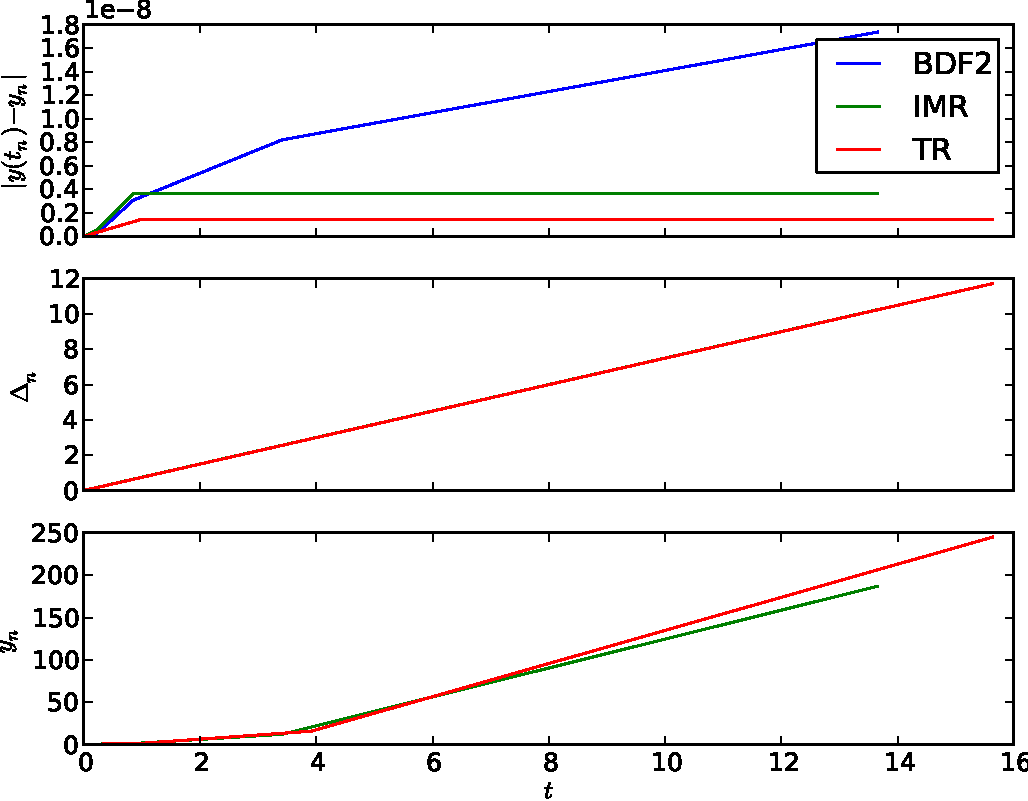
\includegraphics[width=1\textwidth]{plots/aimr_odes/poly2-errornormsvs-dtsvs-tracevaluesvstimes}
  \caption{Absolute error, time step size and computed solutions for the example ODE with exact solution $y(t) = t^2 + 0.5$.}
  \label{fig:imr-poly2-example}
\end{figure}


\subsection{Oscillatory, damped example}
\label{sec:oscill-damp-example}

The next test features a damped oscillatory solution
\begin{equation}
  \label{eqn:imr-test-osc-damp}
  \begin{aligned}
    y(t) &= e^{-\beta t} \sin(\omega t), \\
    f(t,y) &= - \beta e^{-\beta t} \sin(\omega t) + \omega e^{-\beta t} \cos(\omega t).  \end{aligned}
\end{equation} 
The adaptive algorithm should oscillate the step size in time with the oscillating truncation error ($\pd{}{t^3} \sin(t) = -\cos(t)$), while at the same time gradually increasing the step size as the term $e^{-\beta t}$ goes to zero.

??ds write out full lte calculations?

\begin{figure}[h!]
  \centering 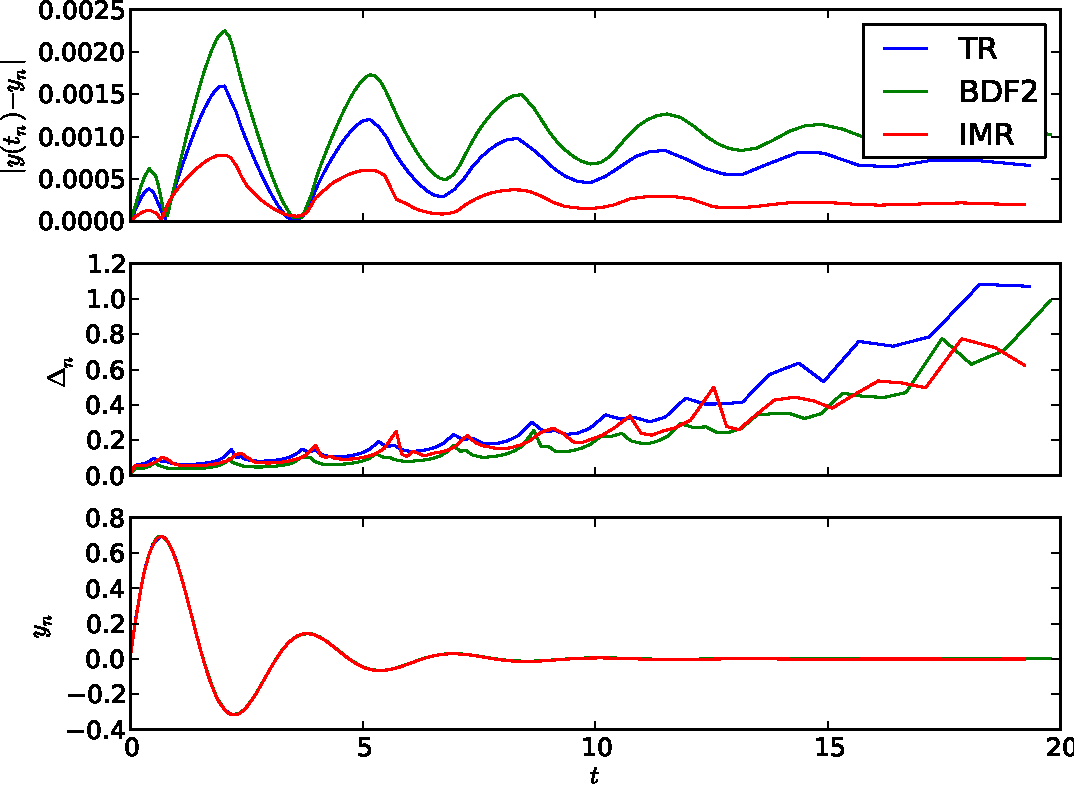
\includegraphics[width=1\textwidth]{plots/aimr_odes/damped_oscillation-errornormsvs-dtsvs-tracevaluesvstimes}
  \caption{Absolute error, time step size and computed solutions for the oscillatory, damped example ODE with exact solution $y(t) = e^{-0.5t} \sin(2\pi t)$.}
  \label{fig:imr-osc-example}
\end{figure}

The ODE was solved with parameters $\omega = 2 \pi$ and $\beta = 0.5$, the results are shown in \autoref{fig:imr-osc-example}.
All three methods have similar errors and time step sizes.
The IMR method choses slighly smaller steps than TR (which probably explains the slightly lower error magnitudes.
BDF2 has the worst errors as expected because its error coefficient is the largest.

Note that the plot shows the global error, whereas local trunction error estimates are used for step size selection calculations.
Hence the fact that the global error increases above the tolerance, $\toltt$, is not suprising.

Interestingly, there is a slight lag on the time step response of the IMR method as time steps become larger.
This could be due to the fact that IMR uses data from three previous steps in its LTE estimate, whereas the others only use two previous steps.

In \autoref{fig:imr-osc-example-scatter} we show plots of the decrease in global error norm as the tolerence is decreased. 
The consistent decrease in the error norms indicates that the all of the adaptive methods are able to control the error in the expected manner.
Plots for the example problems the following Sections are very similar and so are not shown.

\begin{figure}[h!]
  \centering 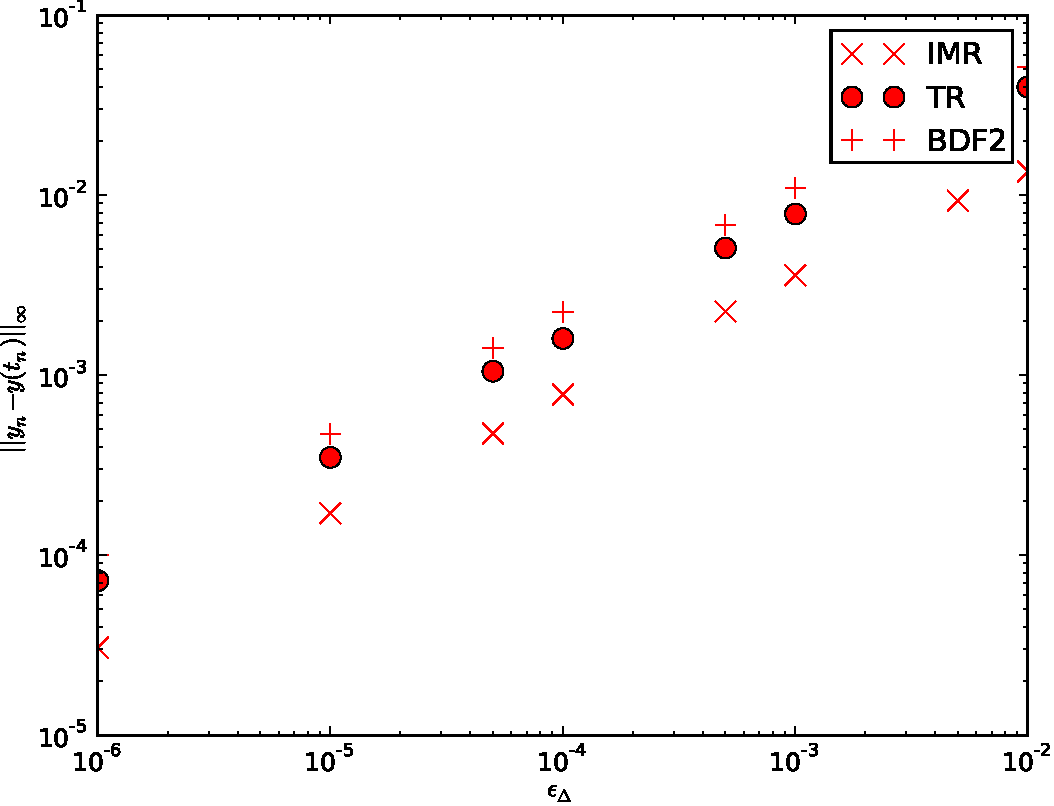
\includegraphics[width=1\textwidth]{plots/aimr_odes/damped_oscillation-maxoferrornormsvs-tol}
  \caption{Behaviour of the global error norm with varying tolerance for the oscillatory, damped example ODE with exact solution $y(t) = e^{-\beta t} \sin(\omega t)$.}
  \label{fig:imr-osc-example-scatter}
\end{figure}

\subsection{Stiff problem}
\label{sec:imr-stiff-example}

We consider stiff example ODE used in the definition of A-stability:
\begin{equation}
  \label{eqn:imr-test-stiff}
  \begin{aligned}
    f(t, \yv) = -\lambda t, \\
  \end{aligned}
\end{equation}
with the exact solution
\begin{equation}
  \label{eqn:imr-test-stiff-exact}
  \yv(t) = e^{-\lambda t} \yv_0. \\
\end{equation} 
This example will test that the single step of the eBDF method provides reliable LTE estimates even in cases of extreme stiffness.
The time steps should start small but rapidly increase as the initial transient decays.

The results of the applying the three methods to problem~\eqref{eqn:imr-test-stiff} with $\lambda = 100$ (fairly stiff) are shown in \autoref{fig:imr-stiff-example}.
The behaviour of the three time integrators is essentially the same, indicating that our adaptivity algorithm is effective for stiff problems.

\begin{figure}[h!]
  \centering
  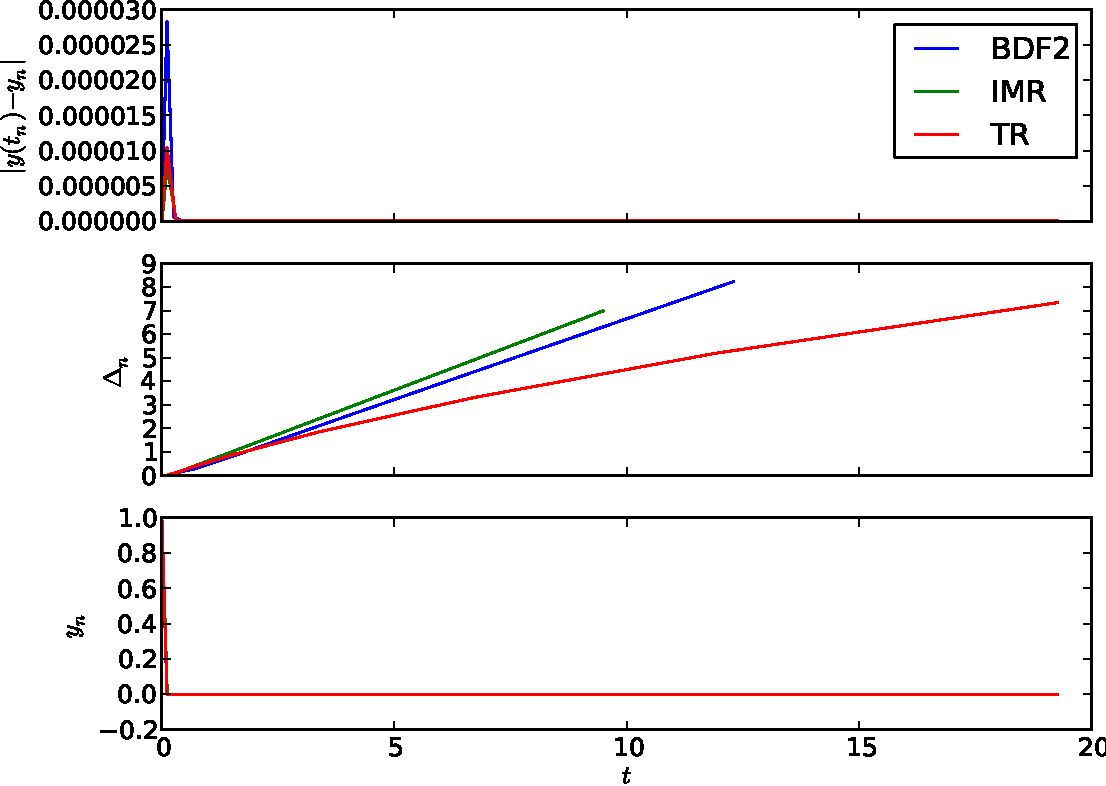
\includegraphics[width=1\textwidth]{plots/aimr_odes/simple_stiff-errornormsvs-dtsvs-tracevaluesvstimes}
  \caption{Absolute error, time step size and computed solutions for the stiff example ODE.}
  \label{fig:imr-stiff-example}
\end{figure}


\subsection{Order reduction example}
\label{sec:order-reduct-example}

\begin{figure}
  \centering  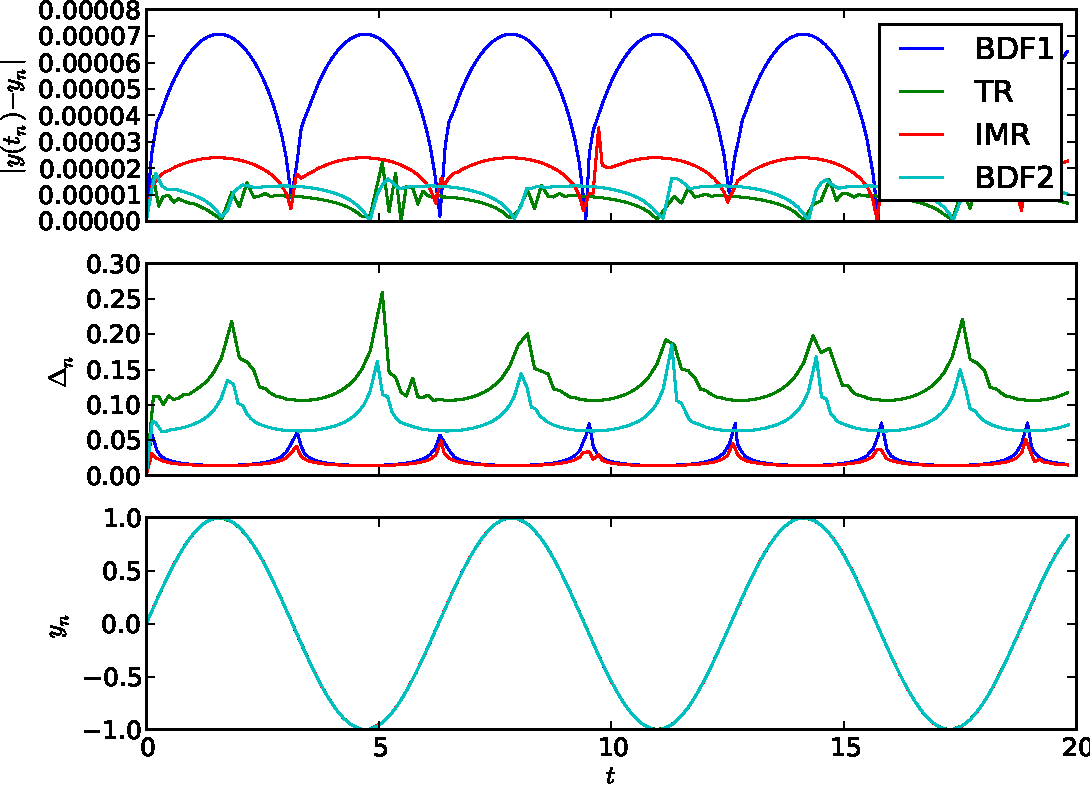
\includegraphics[width=1\textwidth]{plots/aimr_odes/strong_order_reduction-errornormsvs-dtsvs-tracevaluesvstimes}
  \caption{Absolute error, time step size and computed solutions for the stiff order reduction example ODE given in equation~\eqref{eqn:imr-test-order-reduction}
    .}
  \label{fig:imr-order-reduction-example}
\end{figure}

\begin{figure}
  \centering  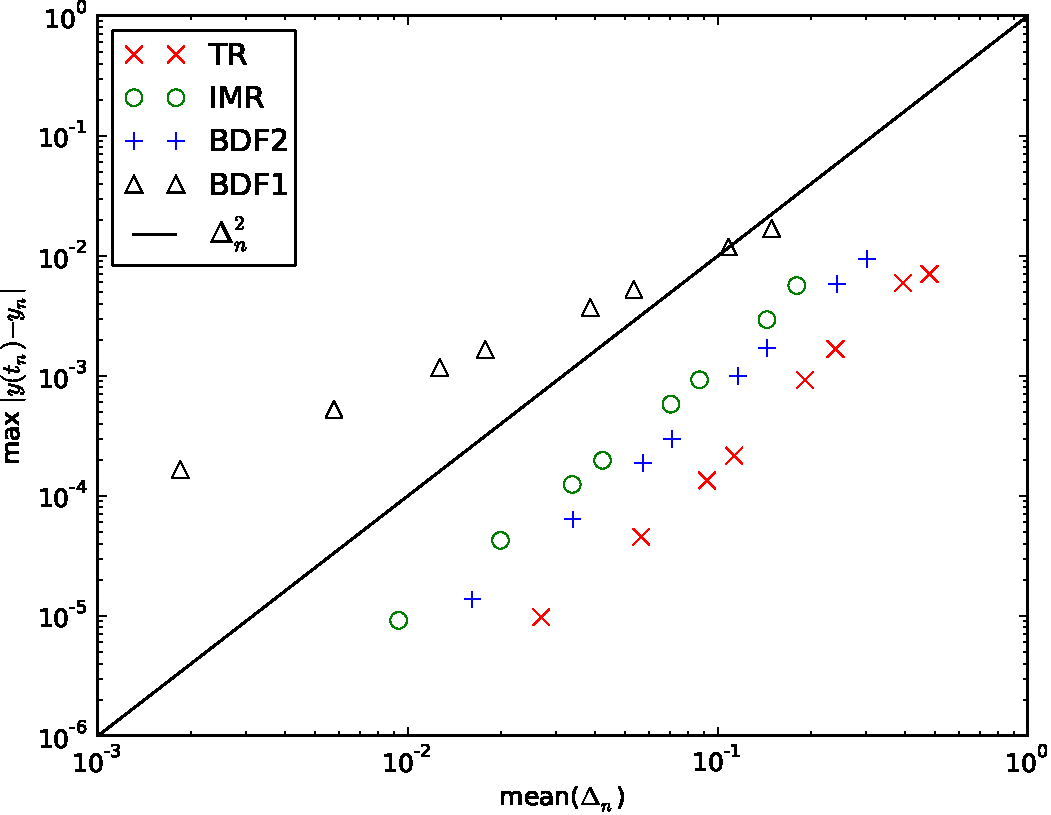
\includegraphics[width=1\textwidth]{plots/aimr_odes/order_reduction-maxoferrornormsvsmeanofdts.pdf}
  \caption{Maximum over time of absolute error vs mean time step for the order reduction example.}
  \label{fig:imr-order-reduction-convergence}
\end{figure}

As a final example we study \eqref{eqn:imr-test-order-reduction}, the test ODE for order reduction discussed in \autoref{sec:order-reduction}.
For these experiments we chose an oscillatory function, $g(t) = \sin(t)$ and $\lambda = 100$.

So, using \eqref{eq:reduced-order-imr-truncation-error}, the dominant term LTE of IMR for the case when $\dtn \gtrsim 0.01$ is
\begin{equation}
  \lte^\imr = \frac{\dtn^2}{4} \sin(\thf),
\end{equation}
for smaller $\dtn$ the $\dtn^3 \cos(t)$ term will gradually become more important.
Note that for TR and BDF2 $\lte \propto \dtn^3 \cos(t)$, while for BDF1 $\lte \propto \dtn^2 \sin(t)$.
Hence we expect to see the adaptive IMR perform similarly to BDF1, and to select much smaller time steps than TR and BDF2 in order to control the larger errors.
To test this we also run the experiment with an adaptive BDF1 (backwards Euler) method using Milne's method for adaptivity.

The results are shown in \autoref{fig:imr-order-reduction-example}. 
As expected the implicit midpoint rule selects time step sizes similarly to the first order BDF1 method due to order reduction.
This allows it to retain similar accuracies to the TR and BDF2 methods at the cost of requiring many more time steps.

The convergence of the solution as $\toltt$ is reduced with fixed $\lambda = 100$ is shown in \autoref{fig:imr-order-reduction-convergence}.
Note that IMR still displays second order convergence (albeit with a much larger constant error). 
This is because we are not increasing $\lambda$ as we decrease $\toltt$, so we measuring the normal convergence not B-convergence.


\section{Additional Notes}

\subsection{Application to Implicit ODEs}
\label{sec:extens-impl-odes}

We sometimes wish to solve a system of equations where $\yv'(t)$ only given implicitly\footnote{This use of ``implicit'' is unrelated to the notion of implicitness in the time integration scheme.} (for example the Gilbert form of the Landau-Lifshitz-Gilbert equation), in this case equation~\eqref{eq:43} becomes
\begin{equation}
  \ffv{t, \yv(t), \yv'(t)} = 0.
\end{equation}

We note that equation~\eqref{eq:basic-midpoint} can also be written in the from
\begin{equation}
  \yv'(\thf) = \frac{\yv_{n+1} - \yv_n}{\dtn} =  \ffv{\thf, \frac{\yv_n + \yv_{n+1}}{2}}.
\end{equation}
The obvious equivalent for IMR is
\begin{equation}
  \ffv{\thf, \frac{\yv_{n+1} + \yv_n}{2}, \frac{\yv_{n+1} - \yv_n}{\dtn}} = 0.
\end{equation}

However the adaptive scheme requires an additional function evaluation.
For implicitly defined functions this is expensive, so this adaptive method is not efficient for equations which can only be defined in such a way.
The LLG can be defined explicitly as well as implicitly so this limitation does not apply in micromagnetics.



\section{Conclusions}

We have implemented an efficent algorithm for adaptive time step selection with the implicit midpoint rule.
The algorithm has been tested on a number of ODEs and found to choose similar time steps to other second order time integrators.
It has also been shown to be robust in stiff problems and to control the error effectively even when order reduction phenomena are encountered.


%%% Local Variables:
%%% mode: latex
%%% TeX-master: "./main"
%%% End:
